% Drafted by moonshotai/kimi-k3.1-pro (Open Math OS worker), 2026-11-13. Not yet human-verified.
% slides_v2.tex: a corrected copy of talk/slides.tex (the working copy of 2026-11-14 23:28, with its
% uncommitted slide "How the AI team worked"), made by Claude Fable 5.2 (AI; a fresh-context agent, brief W054,
% second task), 2026-11-15, so that the deck agrees with report/report.tex. The list of what was wrong is
% talk/SLIDES_VS_REPORT.md (items B-M1 to B-M15, B-R1 to B-R17). Every change is marked by a comment line that
% begins with "v2:". talk/slides.tex itself is unchanged. Not human-reviewed.
\documentclass[aspectratio=169,11pt]{beamer}
\usetheme{default}
\usecolortheme{seahorse}
\setbeamertemplate{navigation symbols}{}
\setbeamertemplate{footline}[frame number]
\setbeamercolor{frametitle}{fg=blue!50!black}
\setbeamercolor{title}{fg=blue!50!black}
\usepackage{amsmath,amssymb}
\usepackage{tikz}
\usetikzlibrary{arrows.meta,positioning}
% colours shared with talk/figures/make_figures.py (symmetric = blue circle, asymmetric = orange square)
\definecolor{symblue}{HTML}{2A78D6}
\definecolor{asymorange}{HTML}{EB6834}
\definecolor{atomgreen}{HTML}{1BAF7A}

% ---- status switches: change these two lines after human sign-off ----
% v2 (B-M8): the switches are set. The written main proof (report, Section 3) is signed by a faculty member
% of the team and its statement is checked by Lean, so the main statement is called "Theorem" and its three
% steps "Lemma"; the footer "candidate proof, under verification" is replaced by nothing. A slide whose
% content has no human reader says so itself (\statusnote, or the red text in its title). The team decides.
\newcommand{\claimstatus}{}
\newcommand{\ourresult}{Theorem}
\newcommand{\ourlemma}{Lemma}
% --------------------------------------------------------------------
\newcommand{\status}{\par\vfill{\tiny\color{gray}\claimstatus\par}}
% v2: an explicit status line for a slide whose content is not human-signed
\newcommand{\statusnote}[1]{\par\vfill{\tiny\color{gray}#1\par}}
% v2 (B-R13 to B-R17): the last five backup slides (balls, polymers, triangles, light, sand) show worked
% examples that are not written in the report. They are left out of the compiled deck. Write \extrabackuptrue
% only after the sentences L-B13 to L-B17 of talk/SLIDES_VS_REPORT.md are in the report.
\newif\ifextrabackup
\extrabackupfalse
\newcommand{\vp}{v_p}
\newcommand{\sd}{s_p}
\newcommand{\Z}{\mathbb{Z}}
\newcommand{\Cq}{C_n^{(q)}}
\DeclareMathOperator{\Fix}{Fix}

\tikzset{
  intnode/.style={circle,draw,fill=black,inner sep=1.4pt},
  symnode/.style={circle,draw=white,fill=symblue,inner sep=2.2pt},
  asymnode/.style={rectangle,draw=white,fill=asymorange,inner sep=2.7pt},
  leafdot/.style={circle,draw,fill=white,inner sep=1.2pt},
  atom/.style={regular polygon,regular polygon sides=3,draw=atomgreen,fill=atomgreen!18,
               inner sep=1pt,minimum size=9mm,font=\small},
  treeedge/.style={draw,thick}
}

\title[Rotations and Fuss--Catalan numbers]%
{The power of $p$ in Fuss--Catalan numbers\\from symmetries of trees}
\subtitle{Caltech Mathathon 2026 --- Problem 137}
\author{Mighty Math Magicians}
\date{15 November 2026}

\usetikzlibrary{shapes.geometric}
\begin{document}

% 1 ------------------------------------------------------------------
\begin{frame}
  \titlepage
  \vspace{-0.5em}
  \centering\footnotesize A counting fact deserves a counting proof.
\end{frame}

% 2 ------------------------------------------------------------------
\begin{frame}{A pattern in the Catalan numbers}
  \begin{columns}[T]
    \column{0.52\textwidth}
      \centering
      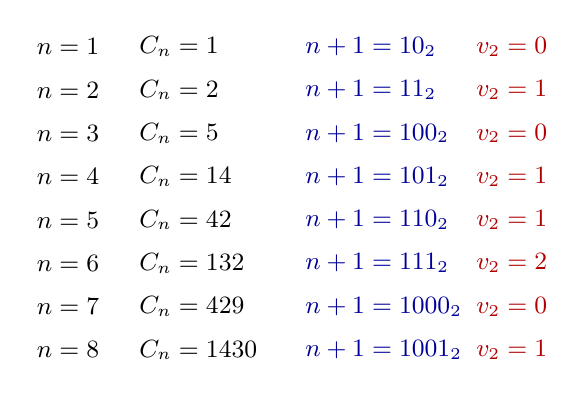
\begin{tikzpicture}[x=0.62cm,y=0.55cm]
        \foreach \x/\n/\c/\b/\e in {
          1/1/1/10/0,
          2/2/2/11/1,
          3/3/5/100/0,
          4/4/14/101/1,
          5/5/42/110/1,
          6/6/132/111/2,
          7/7/429/1000/0,
          8/8/1430/1001/1}
        {
          \node[anchor=west,font=\small] at (0,-\x) {$n=\n$};
          \node[anchor=west,font=\small] at (2.1,-\x) {$C_n=\c$};
          \node[anchor=west,font=\small,blue!60!black] at (5.5,-\x) {$n+1=\b_2$};
          \node[anchor=west,font=\small,red!70!black] at (9.0,-\x) {$v_2=\e$};
        }
      \end{tikzpicture}
    \column{0.44\textwidth}
      \begin{itemize}
        \item $C_n$ counts binary trees with $n$ nodes.
        \item The 2-adic valuation is\\ the number of $1$-bits of $n+1$, minus one.
        \item $C_n$ is \alert{odd} exactly when $n+1$ is a power of $2$.
      \end{itemize}
  \end{columns}
\end{frame}

% 2b (added 2026-11-14 by Claude Fable 5.2; figure: talk/figures/make_figures.py) --------
\begin{frame}{The pattern goes on, for every prime}
  \centering
  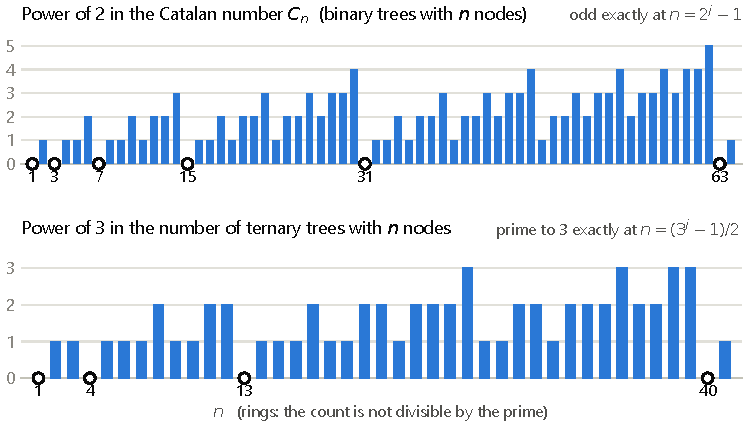
\includegraphics[width=0.76\textwidth]{figures/fig_pattern.pdf}\\[0pt]
  \begin{minipage}{0.93\textwidth}\small
  The power of $p$ is $\bigl(\text{digit sum of the number of leaves in base }p\,-\,1\bigr)/(p-1)$.
  This is known, \emph{by computing with factorials}.
  \textbf{Why should the digits of a number have anything to do with trees?}
  \end{minipage}
\end{frame}

% 2c (added 2026-11-14) ----------------------------------------------
\begin{frame}{A shape of tree is a mobile}
  \centering
  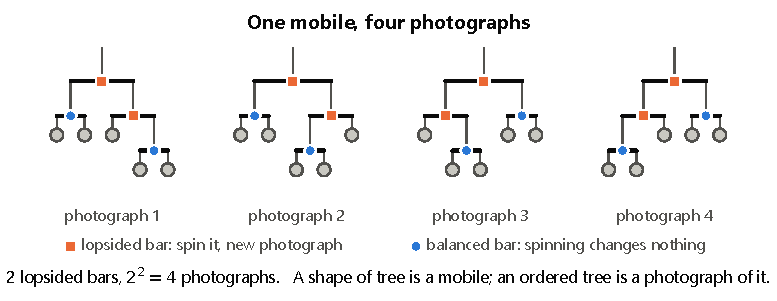
\includegraphics[width=0.9\textwidth]{figures/fig_mobile.pdf}\\[2pt]
  \begin{minipage}{0.95\textwidth}\small
  Every bar can spin. A drawing of a tree is a photograph of the mobile; a mobile with $d$ lopsided bars has
  $p^{d}$ photographs. So the number of drawings is a sum of powers of $p$, one for each mobile, and
  \textbf{its power of $p$ is the smallest one that occurs}, if the number of mobiles with that power is
  not divisible by $p$. That is the plan of the proof.
  \end{minipage}
\end{frame}

% 3 ------------------------------------------------------------------
\begin{frame}{One tree, four sciences}
  \centering
  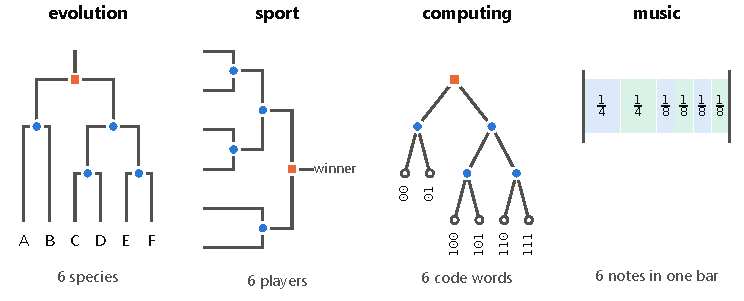
\includegraphics[width=0.88\textwidth]{figures/fig_dialects.pdf}\\[1pt]
  \begin{minipage}{0.96\textwidth}\small
  The left-to-right order of the branches means nothing here: only the \emph{shape} counts.
  \textbf{How many ordered trees stand over one shape? Always a power of $2$.}
  The smallest power that occurs is the power of $2$ in the Catalan number.\\[2pt]
  {\footnotesize $6=110_2$: one node has to be lopsided (orange), and one is enough. Biologists count
  these nodes to measure the balance of an evolutionary tree (Kersting--Fischer 2021).}
  \end{minipage}
\end{frame}

% 3b (added 2026-11-14) ----------------------------------------------
\begin{frame}{Chemistry does it with $p=3$}
  \centering
  % v2 (B-M3): fig_butyl_v2 says "lopsided carbon" where fig_butyl says "asymmetric carbon", which to a
  % chemist means a carbon with four different groups (report, Section 5, item 3; review of the chemistry
  % statements, section 8). One sentence added that says what "lopsided" means.
  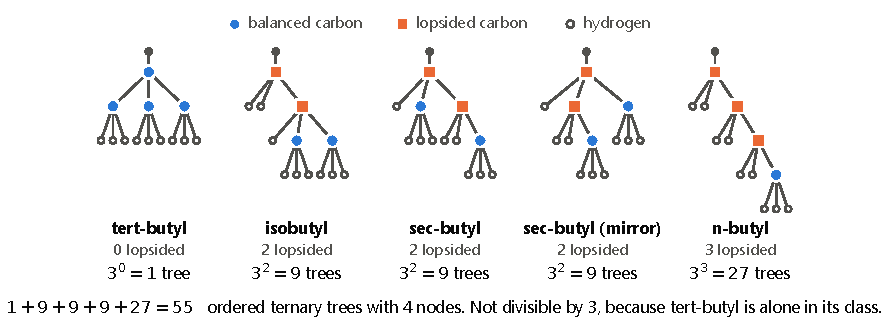
\includegraphics[width=0.96\textwidth]{figures/fig_butyl_v2.pdf}\\[1pt]
  \begin{minipage}{0.96\textwidth}\footnotesize
  The three further bonds of a carbon atom can be \emph{rotated}, not reflected: a cyclic group of
  order $3$ at every node. Ternary trees up to rotation are the alkyl groups, mirror images counted
  separately: $1,1,2,5,11,28,\dots$ (OEIS A000625).
  A carbon is \emph{lopsided} (orange) if its three further branches are not all alike.
  \end{minipage}
\end{frame}

% 3 ------------------------------------------------------------------
\begin{frame}{The problem}
  A \emph{$q$-ary tree}: every node has $q$ ordered branches,
  each empty or again a $q$-ary tree.
  \[
    \Cq=\frac{1}{(q-1)n+1}\binom{qn}{n},\qquad
    m=(q-1)n+1=\#\text{leaves}.
  \]
  \textbf{Known (Konvalinka 2007, via factorials).}
  For $q=p^k$, $p$ prime,
  \[
    \vp\!\bigl(\Cq\bigr)=\frac{\sd(m)-1}{p-1},
  \]
  where $\sd(m)$ is the sum of the base-$p$ digits of $m$.
  \bigskip

  \textbf{Problem 137.} Prove this \alert{from symmetries of trees},
  \emph{without factorial valuations}.
\end{frame}

% 4 ------------------------------------------------------------------
\begin{frame}{Konvalinka's symmetries \dots\ and ours}
  \begin{columns}[T]
    \column{0.48\textwidth}
      \centering\textbf{All permutations}\\[2pt]
      {\small Konvalinka 2007}\\[6pt]
      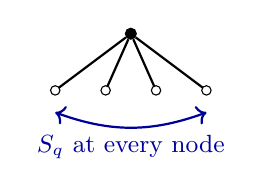
\begin{tikzpicture}[scale=0.8]
        \node[intnode] (r) at (0,0) {};
        \foreach \x/\l in {-1.2/1,-0.4/2,0.4/3,1.2/4}{
          \draw[treeedge] (r) -- (\x,-0.9);
          \node[leafdot] at (\x,-0.9) {};
        }
        \draw[<->,blue!60!black,thick] (-1.2,-1.25) to[bend right=20] (1.2,-1.25);
        \node[blue!60!black,font=\small] at (0,-1.8) {$S_q$ at every node};
      \end{tikzpicture}\\[4pt]
      orbit sizes = products of\\ \textbf{multinomial coefficients}
      \begin{itemize}\small
        \item gives divisibility $p^t\mid\Cq$;
        \item exactness still quoted from factorials.
      \end{itemize}
    \column{0.48\textwidth}
      \centering\textbf{Only rotations}\\[2pt]
      {\small our change}\\[6pt]
      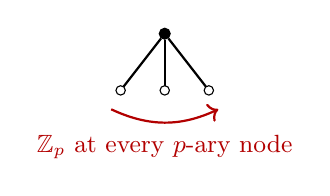
\begin{tikzpicture}[scale=0.8]
        \node[intnode] (r) at (0,0) {};
        \foreach \x in {-0.7,0,0.7}{
          \draw[treeedge] (r) -- (\x,-0.9);
          \node[leafdot] at (\x,-0.9) {};
        }
        \draw[->,red!70!black,thick] (-0.85,-1.2) to[bend right=25] (0.85,-1.2);
        \node[red!70!black,font=\small] at (0,-1.8) {$\Z_p$ at every $p$-ary node};
      \end{tikzpicture}\\[4pt]
      orbit sizes = \textbf{powers of $p$}
      \begin{itemize}\small
        \item a $p$-group (Sylow $p$-subgroup of $S_q$);
        \item minimal orbits can be listed and counted $\bmod\,p$.
      \end{itemize}
  \end{columns}
  \status
\end{frame}

% 5b (added 2026-11-14) ----------------------------------------------
\begin{frame}{Why the smaller group works: bits, not bytes}
  \centering
  % v2 (B-R3): fig_bits_v2 gives the class sizes under all permutations as the report does ("such as 6 and 12")
  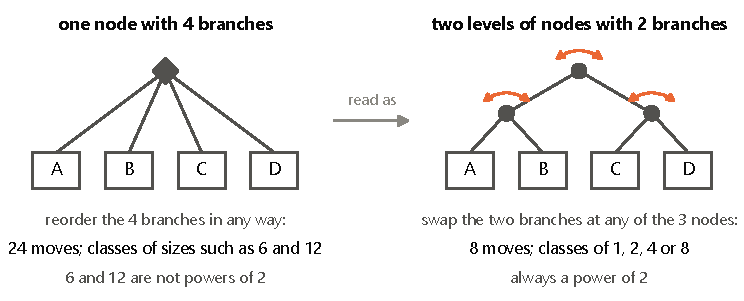
\includegraphics[width=0.9\textwidth]{figures/fig_bits_v2.pdf}\\[5pt]
  \begin{minipage}{0.93\textwidth}\small
  For $q=p^k$: read every $q$-ary node as $k$ levels of $p$-ary nodes, and only \emph{rotate} at each of them.
  Then every class of trees has $p^{d}$ members, where $d$ is the number of asymmetric nodes.
  \end{minipage}
\end{frame}

% 5c (added 2026-11-14) ----------------------------------------------
\begin{frame}{Prime powers in a picture: cut a square ($q=4$)}
  \centering
  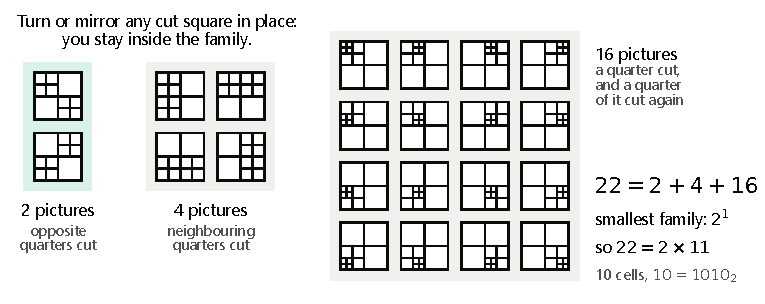
\includegraphics[width=0.9\textwidth]{figures/fig_quadtree.pdf}\\[1pt]
  \begin{minipage}{0.95\textwidth}\small
  The $8$ symmetries of a square permute its four quarters and keep the diagonals together: exactly our
  group for a node with four branches. All families have a power of $2$ members; the smallest one gives
  the power of $2$ in the count. {\footnotesize (Cutting squares this way is how quadtrees store images.)}
  \end{minipage}
\end{frame}

% 5 ------------------------------------------------------------------
\begin{frame}{Step 0: a $q$-ary tree is a $p$-ary tree}
  \begin{columns}[T]
    \column{0.46\textwidth}
      \centering
      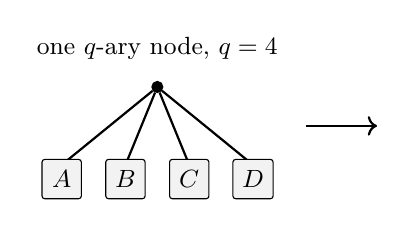
\begin{tikzpicture}[scale=0.9]
        % q-ary node (q=4) and its p-ary block (p=2,k=2)
        \node[intnode] (r) at (0,0) {};
        \foreach \x/\c in {-1.35/A,-0.45/B,0.45/C,1.35/D}{
          \draw[treeedge] (r) -- (\x,-1.1);
          \node[draw,rounded corners=1pt,fill=gray!10,minimum size=5mm,font=\small]
            at (\x,-1.3) {$\c$};
        }
        \node[font=\small] at (0,0.55) {one $q$-ary node, $q=4$};
        \draw[->,thick] (2.1,-0.55) -- (3.1,-0.55);
      \end{tikzpicture}
    \column{0.5\textwidth}
      \centering
      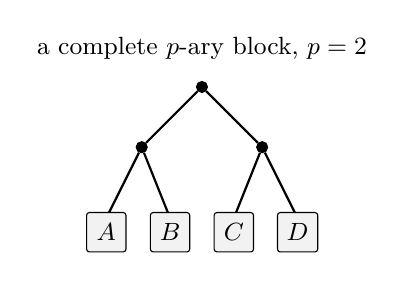
\begin{tikzpicture}[scale=0.9]
        \node[intnode] (r) at (0,0) {};
        \node[intnode] (l) at (-0.85,-0.85) {};
        \node[intnode] (rr) at (0.85,-0.85) {};
        \draw[treeedge] (r) -- (l); \draw[treeedge] (r) -- (rr);
        \foreach \p/\x/\c in {l/-1.35/A,l/-0.45/B,rr/0.45/C,rr/1.35/D}{
          \draw[treeedge] (\p) -- (\x,-1.85);
          \node[draw,rounded corners=1pt,fill=gray!10,minimum size=5mm,font=\small]
            at (\x,-2.05) {$\c$};
        }
        \node[font=\small] at (0,0.55) {a complete $p$-ary block, $p=2$};
      \end{tikzpicture}
  \end{columns}
  \bigskip
  Replace each node by a complete $p$-ary tree of height $k$ ($p^k=q$ branches).
  \begin{itemize}
    \item Bijection: $q$-ary trees $\longleftrightarrow$ $p$-ary trees
          whose leaves all sit at \alert{depth divisible by $k$}.
    \item Leaf count unchanged: $m=(q-1)n+1$.
    % v2 (B-M12): the item "The answer can only depend on $m$." is removed: it does not follow at this step
    % (the set of trees depends on k as well), and it is not in the report.
  \end{itemize}
\end{frame}

% 6 ------------------------------------------------------------------
\begin{frame}{Step 1: rotate, don't permute}
  \begin{columns}[T]
    \column{0.55\textwidth}
      \centering
      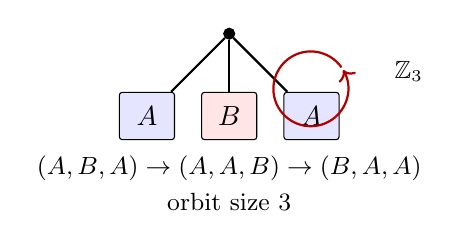
\begin{tikzpicture}[scale=0.95]
        \node[intnode] (r) at (0,0) {};
        \node[draw,rounded corners=1pt,fill=blue!10,minimum width=7mm,minimum height=6mm] (a) at (-1.1,-1.1) {$A$};
        \node[draw,rounded corners=1pt,fill=red!10,minimum width=7mm,minimum height=6mm] (b) at (0,-1.1) {$B$};
        \node[draw,rounded corners=1pt,fill=blue!10,minimum width=7mm,minimum height=6mm] (c) at (1.1,-1.1) {$A$};
        \draw[treeedge] (r) -- (a); \draw[treeedge] (r) -- (b); \draw[treeedge] (r) -- (c);
        \draw[->,thick,red!70!black] (1.5,-0.45) arc[start angle=35,end angle=390,radius=0.5];
        \node[font=\small] at (2.4,-0.5) {$\Z_3$};
        \node[font=\small,align=center] at (0,-2.0)
          {$(A,B,A)\to(A,A,B)\to(B,A,A)$\\[2pt] orbit size $3$};
      \end{tikzpicture}
    \column{0.41\textwidth}
      At each node, cyclically rotate the $p$ subtrees.
      \begin{itemize}
        \item Generates a $p$-group.
        \item Rotations preserve leaf depths, so the class condition survives.
        \item $\sim$ = equivalence generated by these moves.
      \end{itemize}
  \end{columns}
  \bigskip
  \begin{block}{Key definition}
    A node is \textcolor{blue!60!black}{\textbf{symmetric}} if its $p$ subtrees
    are pairwise equivalent, \textcolor{red!70!black}{\textbf{asymmetric}} otherwise.\\
    $d(T)=\#\{$asymmetric nodes of $T\}$.
  \end{block}
\end{frame}

% 7 ------------------------------------------------------------------
\begin{frame}{Class size $=p^{d(T)}$}
  \centering
  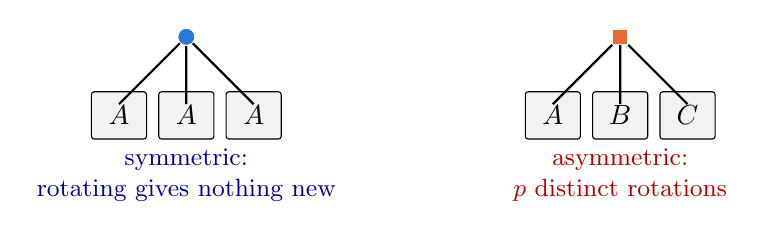
\begin{tikzpicture}[scale=0.95]
    % symmetric node (blue)
    \node[symnode] (s) at (-3.2,0) {};
    \node[draw,rounded corners=1pt,fill=gray!10,minimum width=7mm,minimum height=6mm] at (-4.1,-1.05) {$A$};
    \node[draw,rounded corners=1pt,fill=gray!10,minimum width=7mm,minimum height=6mm] at (-3.2,-1.05) {$A$};
    \node[draw,rounded corners=1pt,fill=gray!10,minimum width=7mm,minimum height=6mm] at (-2.3,-1.05) {$A$};
    \draw[treeedge] (s) -- (-4.1,-0.9); \draw[treeedge] (s) -- (-3.2,-0.9); \draw[treeedge] (s) -- (-2.3,-0.9);
    \node[blue!60!black,font=\small,align=center] at (-3.2,-1.85) {symmetric:\\rotating gives nothing new};
    % asymmetric node (red)
    \node[asymnode] (a) at (2.6,0) {};
    \node[draw,rounded corners=1pt,fill=gray!10,minimum width=7mm,minimum height=6mm] at (1.7,-1.05) {$A$};
    \node[draw,rounded corners=1pt,fill=gray!10,minimum width=7mm,minimum height=6mm] at (2.6,-1.05) {$B$};
    \node[draw,rounded corners=1pt,fill=gray!10,minimum width=7mm,minimum height=6mm] at (3.5,-1.05) {$C$};
    \draw[treeedge] (a) -- (1.7,-0.9); \draw[treeedge] (a) -- (2.6,-0.9); \draw[treeedge] (a) -- (3.5,-0.9);
    \node[red!70!black,font=\small,align=center] at (2.6,-1.85) {asymmetric:\\$p$ distinct rotations};
  \end{tikzpicture}
  \bigskip

  % v2 (B-M8): \ourlemma in place of \ourresult (Lemma 3.12 of the report)
  \begin{block}{\ourlemma\ (class size)}
    $|[T]|=p^{d(T)}$, by induction: the $p$ rotations of a word of length $p$
    are all equal or pairwise distinct, because $p$ is prime.
  \end{block}
  \[
    \Cq=\sum_{\text{rotation classes}}p^{\,d}
    \;\Longrightarrow\;
    \vp(\Cq)\ge \min d,\qquad
    \Cq/p^{\min d}\equiv N_{\min}\pmod p .
  \]
  \status
\end{frame}

% 8 ------------------------------------------------------------------
\begin{frame}{Step 2: every class has at least $p^t$ trees}
  % v2 (B-M8): \ourlemma in place of \ourresult (Proposition 3.14 of the report)
  \begin{block}{\ourlemma\ (lower bound)}
    Every $p$-ary tree $T$ with $m$ leaves has
    \[
      d(T)\ \ge\ t:=\frac{\sd(m)-1}{p-1}.
    \]
  \end{block}
  Only two digit facts, \textbf{no factorials}:
  \[
    \sd(pa)=\sd(a),\qquad
    \sd(a+b)\le\sd(a)+\sd(b)\ \text{(equality: no carries)}.
  \]
  Induction on $T=(T_1,\dots,T_p)$, $m_i$ leaves in $T_i$:
  \begin{itemize}
    \item \textcolor{blue!60!black}{Symmetric root}: all $m_i$ equal, $m=pm_1$, and
          $d=p\,d(T_1)\ge p\,t(m_1)\ge t(m)$.
    \item \textcolor{red!70!black}{Asymmetric root}:
          $d=1+\sum_i d(T_i)\ge 1+\sum_i t(m_i)\ge t(m)$.
  \end{itemize}
  Hence $p^t\mid\Cq$: Konvalinka's divisibility, now a five-line induction.
\end{frame}

% 8b (optional; added 2026-11-14 by Claude Fable 5.2: the same step, said with carries) ----
\begin{frame}{Step 2 again: the carry budget \hfill\normalsize\textcolor{red!70!black}{same statement, a second way to see it}}
  \centering
  % v2 (B-M15): fig_carry_budget_v2 says "a most symmetric tree with 7 leaves" (there are three), not "the".
  % (B-R5: the two trees with 7 leaves are an example of Facts 1 to 3 of Section 4.4 of the report; the
  % example itself is not written in the report, whose example has 13 leaves.)
  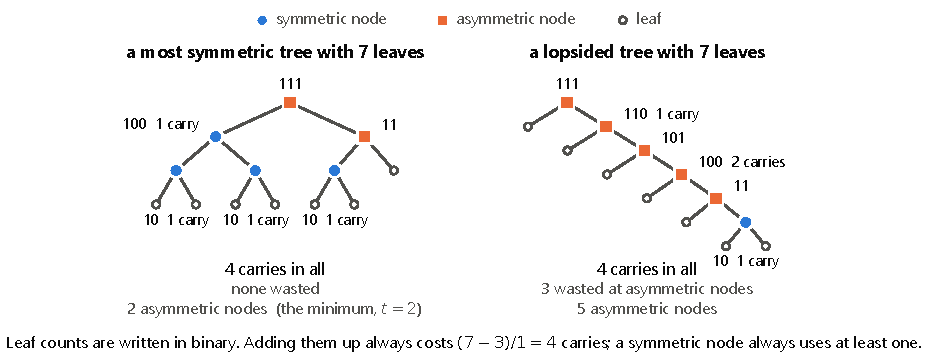
\includegraphics[width=0.92\textwidth]{figures/fig_carry_budget_v2.pdf}\\[2pt]
  \begin{minipage}{0.96\textwidth}\small
  A carry is one trade of $p$ units for $1$ unit in the next column. \textbf{Every} tree with $m$ leaves
  makes $\nu(m)=\frac{m-\sd(m)}{p-1}$ of them. A symmetric node always makes at least one. So at most
  $\nu(m)$ of the $\frac{m-1}{p-1}$ nodes are symmetric: $d(T)\ge\frac{m-1}{p-1}-\nu(m)=t$.
  Equality: no carry is wasted. That is Step~3.
  \end{minipage}
  % v2 (B-M8): this argument is not human-signed (report, Section 4.4), so the slide says so
  \statusnote{this second argument: checked by one AI referee and by Lean; no human has read it}
\end{frame}

% 9 ------------------------------------------------------------------
\begin{frame}{Step 3: minimal trees are built from the digits of $m$}
  \textbf{Minimal} means $d(T)=t$: the smallest classes, size $p^t$.
  \bigskip

  Tracing equality through the induction forces:
  \begin{itemize}
    \item every internal node \textcolor{red!70!black}{asymmetric}
          (the \emph{skeleton}, $t$ nodes);
    \item hanging from it, \textbf{complete trees} of height $j$ --- \emph{atoms};
    \item \alert{no carries} at every node $\Rightarrow$
          exactly $m_j$ atoms of height $j$:\\
          \centering\textbf{the atoms are the base-$p$ digits of $m$.}
  \end{itemize}
  \bigskip
  % v2 (B-M8): \ourlemma in place of \ourresult (Proposition 3.19 of the report)
  \begin{block}{\ourlemma\ (skeleton bijection)}
    Minimal classes $\longleftrightarrow$ cyclic skeleton trees on the digit atoms,
    an atom of height $j$ sitting at depth $\equiv -j \pmod k$.
  \end{block}
  \status
\end{frame}

% 9b (added 2026-11-14) ----------------------------------------------
\begin{frame}{The answer in one picture}
  \centering
  % v2 (B-M15, B-R6): fig_atoms_v2 says "A most symmetric tree with 13 leaves" (there are three; report,
  % Section 5, item 6) and no longer prints the value of C_12, which is not in the report. The sentence
  % below is changed in the same way; "one for each unit of each digit" is the report's wording.
  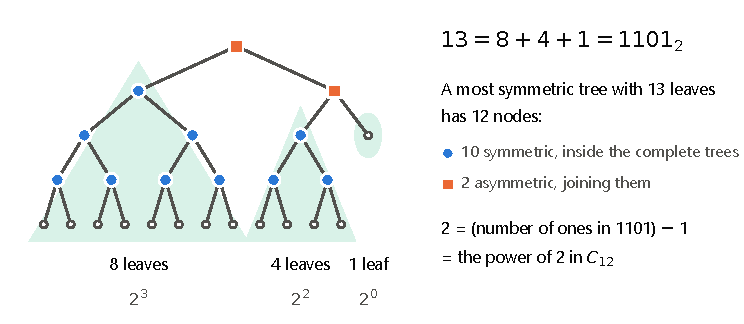
\includegraphics[width=0.93\textwidth]{figures/fig_atoms_v2.pdf}\\[3pt]
  \begin{minipage}{0.93\textwidth}\small
  A most symmetric tree is made of complete trees, one for each unit of each base-$p$ digit of $m$.
  The digits are not a formula here: \textbf{they are the building blocks.}
  \end{minipage}
  \status
\end{frame}

% 10 -----------------------------------------------------------------
\begin{frame}{Running example: $p=2$, $n=6$}
  \[
    C_6=132=2^2\cdot 33,\qquad m=7=111_2,\qquad t=2 .
  \]
  Atoms of heights $0,1,2$: triangles with $1,2,4$ leaves.
  The three minimal skeletons (unordered binary trees on the atoms):
  \begin{center}
  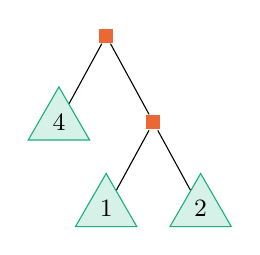
\begin{tikzpicture}[level distance=11mm,sibling distance=12mm]
    \node[asymnode]{}
      child{node[atom]{4}}
      child{node[asymnode]{}
        child{node[atom]{1}} child{node[atom]{2}}};
  \end{tikzpicture}
  \qquad
  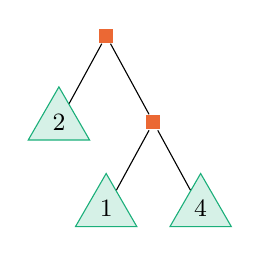
\begin{tikzpicture}[level distance=11mm,sibling distance=12mm]
    \node[asymnode]{}
      child{node[atom]{2}}
      child{node[asymnode]{}
        child{node[atom]{1}} child{node[atom]{4}}};
  \end{tikzpicture}
  \qquad
  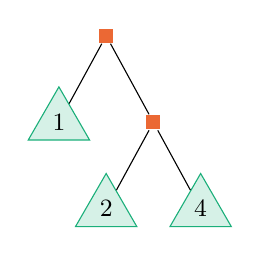
\begin{tikzpicture}[level distance=11mm,sibling distance=12mm]
    \node[asymnode]{}
      child{node[atom]{1}}
      child{node[asymnode]{}
        child{node[atom]{2}} child{node[atom]{4}}};
  \end{tikzpicture}
  \end{center}
  \begin{itemize}
    % v2 (B-M10): "together $132=4\cdot 33$" read as if the three classes held all 132 trees.
    \item Each of these three classes has $2^2=4$ trees: $12$ of the $132$. And $132/4=33$ is odd.
    \item $11$ rotation classes in all, $N_{\min}=3$ (odd).
    % v2 (B-R7): "These are the rooted phylogenetic trees on the three $1$-bits of $7$." is not in the report;
    % replaced by the sentence of its Example 3.28.
    \item The three skeletons differ by the atom that hangs at the root.
  \end{itemize}
  \status
\end{frame}

% 11 -----------------------------------------------------------------
\begin{frame}{Step 4: a carry is a collapsing cherry}
  Count minimal classes $\bmod\,p$ by cycling $p$ same-class labels:
  only \textbf{fixed} trees survive $\bmod\,p$ --- and those have a \emph{cherry}.
  \begin{center}
  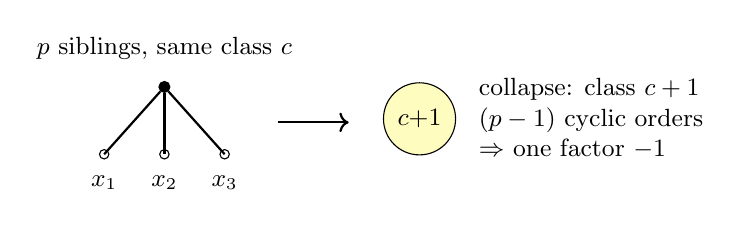
\begin{tikzpicture}[scale=0.9]
    % cherry -> single atom
    \node[intnode] (v) at (0,0) {};
    \foreach \x/\l in {-0.85/x_1,0/x_2,0.85/x_3}{
      \node[leafdot] at (\x,-0.95) {};
      \node[font=\small] at (\x,-1.35) {$\l$};
      \draw[treeedge] (v) -- (\x,-0.95);
    }
    \node[font=\small] at (0,0.55) {$p$ siblings, same class $c$};
    \draw[->,thick] (1.6,-0.5) -- (2.6,-0.5);
    \node[draw,circle,fill=yellow!25,minimum size=6mm,font=\small] at (3.6,-0.45) {$c{+}1$};
    \node[font=\small,align=left,anchor=west] at (4.3,-0.45) {collapse: class $c+1$\\
      $(p-1)$ cyclic orders\\ $\Rightarrow$ one factor $-1$};
  \end{tikzpicture}
  \qquad
  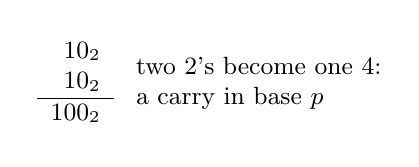
\begin{tikzpicture}[scale=0.75]
    % column addition 2+2 = 4
    \node[font=\small] at (0,0) {$\begin{array}{r}10_2\\10_2\\ \hline 100_2\end{array}$};
    \node[font=\small,align=left] at (3.1,0) {two $2$'s become one $4$:\\
      a \alert{carry} in base $p$};
  \end{tikzpicture}
  \end{center}
  \[
    T(a)\equiv -T(a-p\,e_c+e_{c+1})\pmod p,\qquad
    \text{carries end at one leaf}\;\Rightarrow\;T(a)\equiv(-1)^t .
  \]
  % v2 (B-R8): the chain $T(3)\equiv -T(2)\equiv T(1)=1$ is not written in the report; the line now says
  % what its Example 3.28 says.
  Running example: $t=2$ carries, so $N_{\min}\equiv(-1)^2=1\pmod 2$; and indeed $N_{\min}=3$.
  \status
\end{frame}

% 12 -----------------------------------------------------------------
\begin{frame}{Conclusion: exact valuation, plus the residue}
  \begin{block}{\ourresult\ (main statement)}
    For every prime power $q=p^k$,
    \[
      \vp\!\bigl(\Cq\bigr)=\frac{\sd(m)-1}{p-1},
      \qquad m=(q-1)n+1,
    \]
    and, writing $m=\sum_j m_jp^j$ in base $p$,
    \[
      \frac{\Cq}{p^t}\equiv\frac{(-1)^t}{\prod_j m_j!}\pmod p .
    \]
  \end{block}
  % v2 (B-M2): one item added, in the words of the report ("The result on one page"; Section 1.4); the list
  % is set in \small so that the frame still fits.
  \begin{itemize}\small\setlength{\itemsep}{1pt}
    \item Class sizes $p^d$ with $d\ge t$; the sum $\bmod\,p$ sees only minimal classes.
    \item Their number is $\equiv(-1)^t/\prod_j m_j!\not\equiv 0\pmod p$.
    \item No valuation of a factorial, binomial or multinomial is used.
    \item Both formulas are known as statements; ours is the proof from tree symmetries.
  \end{itemize}
  \status
\end{frame}

% 13 -----------------------------------------------------------------
\begin{frame}{A prime-power example: $p=2$, $q=4$, $n=4$}
  \[
    C_4^{(4)}=140=2^2\cdot 35,\qquad m=13=1101_2,\qquad t=2 .
  \]
  Atoms of heights $0,2,3$ (sizes $1,4,8$); leaf depths must be \textbf{even}
  ($k=2$). Only one skeleton fits:
  \begin{center}
  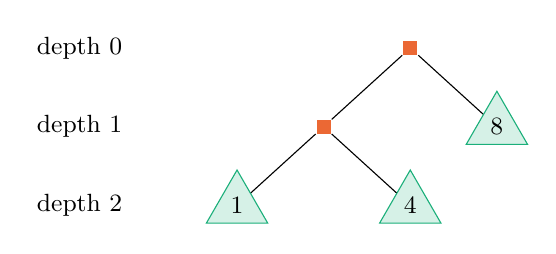
\begin{tikzpicture}[level distance=10mm,sibling distance=22mm]
    \node[asymnode]{}
      child{node[asymnode]{}
        child{node[atom]{1}} child{node[atom]{4}}}
      child{node[atom]{8}};
    \node[font=\small] at (-4.2,0) {depth $0$};
    \node[font=\small] at (-4.2,-1.0) {depth $1$};
    \node[font=\small] at (-4.2,-2.0) {depth $2$};
  \end{tikzpicture}
  \end{center}
  \begin{itemize}
    \item Atom $8$ (height $3$) at depth $1$; atoms $1$, $4$ (heights $0$, $2$) at depth $2$:
          height $+$ depth is even each time.
    \item Carries: $(2,1)\to(0,2)\to(1,0)$, two carries, sign $+1$.
          So $N_{\min}=1$, and indeed $140/4=35$ is odd.
  \end{itemize}
  \status
\end{frame}

% 14 -----------------------------------------------------------------
% v2 (B-M4): in the report the closed families (C11) and the level profiles (C10) are proved (Section 4.5)
% and checked by Lean; only the weighted theorem with the rotation group (C9) is a conjecture. The slide said
% "conjecture" for all three and "not yet proved". The items are in the report's order now (the level
% profiles follow from the closed families), one sentence on invariant weights (C28, same section) is added,
% and the status is the report's: written on the last night, read by no human, not claimed as new. They are
% not called theorems, because no human has signed them.
\begin{frame}{What else falls out \hfill\normalsize\textcolor{red!70!black}{two proved (by AI and Lean only), one conjecture}}
  \begin{itemize}
    \item \textbf{Any closed family.}
      For any rotation-closed family $F$ of trees with $m$ leaves:
      $p^t\mid|F|$ and $|F|/p^t\equiv\#\{\text{minimal classes in }F\}\pmod p$.
      Also $p^t$ divides the sum over $F$ of any integer weight that rotations do not change.
      \par\hfill{\small(C11, C28: proved in the report, Section 4.5; checked by Lean)}
    \item \textbf{Level profiles.}
      Rotations preserve the number $n_i$ of nodes at each depth, so $p^t$
      divides $\prod_i\binom{q n_i}{n_{i+1}}$ for every profile with $\sum n_i=n$.
      \par\hfill{\small(C10: proved in the report, Section 4.5; checked by Lean)}
    \item \textbf{Weighted Fuss--Catalan numbers.}
      Konvalinka's weighted theorem seems to need only transitivity on the $q$
      branches; our rotation group is transitive, so the weighted theorem should
      also become free of factorial valuations.
      \par\hfill{\small(conjecture C9; computed for six values of $q$, not proved)}
  \end{itemize}
  \vfill
  {\small The two proofs are a few lines from Steps~1 and~2. They were written on the last night and no
  human has read them; no search of the literature was made, and we do not claim that the statements are new.
  Computed beforehand: every level profile up to $22$ nodes for $q=2$ (up to $12$--$15$ for $q=3,4,5,8,9$).}
\end{frame}

% 14b ----------------------------------------------------------------
\begin{frame}{Why the most symmetric shapes decide}
  \centering
  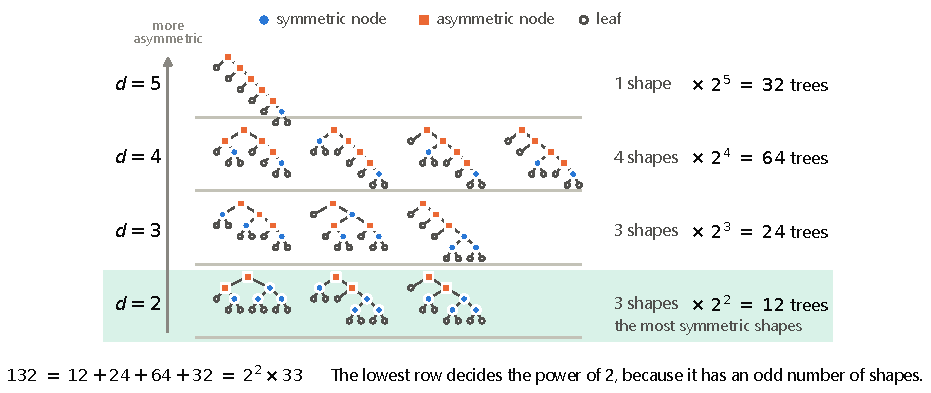
\includegraphics[width=0.86\textwidth]{figures/fig_levels.pdf}\\[1pt]
  \begin{minipage}{0.95\textwidth}\small
  For $2$-adic eyes $2^d$ is \emph{small} when $d$ is large, so the lowest row decides.
  A physicist would say: \textbf{the valuation is the ground-state energy}, and we must check that the number
  of ground states does not vanish modulo $p$.
  % v2 (B-M13): "this is literal" and "$16$ is the largest symmetry factor" went beyond the report (Section 5,
  % item 7: an analogy over exact arithmetic; the role of 16 depends on how the coupling is written).
  {\footnotesize For $p=2$ the arithmetic is that of the tree
  diagrams of a cubic field theory, each divided by its symmetry factor $2^{\#\text{symmetric}}$:
  $\tfrac3{16}+\tfrac38+\tfrac44+\tfrac12=\tfrac{33}{16}=C_6/2^6$.}
  \end{minipage}
\end{frame}

% v2 (B-M9): the title said "Two more proofs ... checked by computer and by AI referees, not yet by us".
% The report (Sections 2.3 and 4.1 to 4.3) has three further proofs, and their status differs: the
% lattice-path proof was read and verified by a faculty member of the team and is checked by Lean; the
% algebraic proof is checked by Lean and by one AI referee and has no human reader; the accounting proof was
% read by the faculty member and is not signed. The lattice-path proof is added in four lines (statements of
% Sections 1.4 and 4.1 of the report), each proof gets its status in grey, and the frame is set in \small so
% that it still fits. The texts of "Algebra only" and "Accounting" are unchanged apart from the type size
% and one note in brackets: that $y$ marks asymmetric nodes is, in the report, a reading confirmed by
% computation only.
\begin{frame}{Three more proofs \hfill\normalsize\textcolor{red!70!black}{who has checked each is said in grey}}
  \small
  \textbf{Lattice paths.} The same plan for words in two letters, with rotations of nested blocks of
  $p$-power length. It proves Kummer's theorem with its residue; our case follows from
  $\binom{qn+1}{n}=(qn+1)\,\Cq$. The method is known (Smith 1993, Wildon 2016), and it acts on paths, not on trees.
  {\footnotesize\textcolor{gray}{Read and verified by a faculty member of the team; checked by Lean.}}

  \textbf{Algebra only.} Trees by number of leaves: $G=x+G^q$.
  For every series, $f^p=f(x^p)+p\cdot\theta(f)$. Replace that $p$ by a variable $y$ (shown for $q=p$):
  \[ F=x+F(x^p,y^p)+y\,\theta(F). \]
  {\footnotesize $y$ marks asymmetric nodes.\quad $y=p$: ordered trees.\quad $y=1$: shapes.\quad
  $y=0$: only the complete trees, $x+x^p+x^{p^2}+\cdots$\quad
  (For $p=2$ this equation is Etherington's, 1939. That $y$ marks asymmetric nodes was confirmed by
  computation only; the proof does not use it.)}\\[2pt]
  Digit sums give the lowest power $y^t$; a derivative identity modulo $p$ gives its coefficient.
  No tree, no formula for factorials; it shares no lemma with the main proof.
  {\footnotesize\textcolor{gray}{Checked by Lean and by one AI referee; no human has read it.}}

  \textbf{Accounting.} Label the leaves: each of the $\frac{m-1}{p-1}$ nodes is worth
  $-p$, and $m!$ absorbs $\frac{m-\sd(m)}{p-1}$ of them:\quad
  $\Cq\cdot\prod_j m_j!\equiv(-p)^{\,t}\pmod{p^{\,t+1}}$.
  {\footnotesize\textcolor{gray}{Read by a faculty member, not signed. It uses the carry step of the main proof.}}
\end{frame}

% 15 -----------------------------------------------------------------
\begin{frame}{The idea in one sentence}
  \centering\Large
  Shrink the symmetry group until it is a $p$-group.\\[8pt]
  Then orbit sizes are powers of $p$,\\[4pt]
  the smallest orbits are built from the digits of $m$,\\[4pt]
  and a carry in base $p$ is a cherry collapsing.\\[14pt]
  \normalsize
  % v2 (B-R9): "Exactness --- not just divisibility --- comes free." is not in the report, and exactness is
  % what the count of Step 4 pays for.
  Exactness --- not just divisibility --- comes from counting the smallest orbits modulo $p$.
\end{frame}

% 16 -----------------------------------------------------------------
% v2 (B-M5, B-M6, B-M14, B-R10): this frame is rewritten from Sections 2.3, 7, 9.1, 9.2 and 9.4 of the
% report. What was wrong: "these slides by Kimi" and "independent re-check, literature scan, explainer ... by
% other logged worker models (Mistral Large 4.0, Muse Spark Open, DeepSeek Flash)" (the replication, the
% literature scan and the explainer were Kimi's; DeepSeek Flash did a connectivity test only; the three
% further proofs, the figures and most programs are Claude Fable 5.2's); "explainer" (not in the report);
% "23 smaller ones" (10, then 13 smaller ones); the Lean item (one proof, for q = 2 in Mathlib's terms:
% now three proofs, for every q, on the required versions); "What humans verified: to be filled in".
% The frame is set in \footnotesize so that it fits.
% One clause is from AI_USAGE.md and the comments of this file, not from Section 9.1 of the report:
% that the slides were revised by Claude Fable 5.2.
\begin{frame}{How AI was used}
  \footnotesize
  \begin{itemize}\setlength{\itemsep}{2pt}
    \item \textbf{The idea of the main proof:} Claude Fable 5.2 (the orchestrating session).
    \item \textbf{Writing:} the first \LaTeX\ write-up of the main proof, a replication of the checks, the
      literature scan and a first draft of these slides: Kimi K3.1 Pro (Open Math OS). The three further
      proofs, most programs, the figures and the revision of the slides: Claude Fable 5.2, in several
      sessions (the question behind the lattice-path proof was a team member's). The next slide:
      Claude Opus 5.5.
    \item \textbf{Attacking the main proof:} three review rounds. Mistral Large 4.0, Muse Spark Open
      and a separate run of Kimi K3.1 Pro found $14$ defects in the write-up; a line-by-line
      read by Claude found $4$ more; two further Claude referees who had seen none
      of our notes found $10$, then $13$ smaller ones. No counterexample in any round; all
      repaired. Computer checks: every tree for small sizes, then $1067$ leaf counts
      up to about $400$ leaves, no failures.
    \item \textbf{Checked by Lean 4} (Lean v4.35.0, Mathlib v4.35.0, no \texttt{sorry}): three proofs (the
      main proof, lattice paths, algebra), valuation and residue for every $q=p^k$, stated with Mathlib's
      own binomial coefficient. Lean files by Claude Fable 5.2, Kimi K3.1 Pro and, for one file,
      Mistral Large 4.0.
    \item \textbf{What people on the team verified:} a faculty member looked through the main proof and
      judged it good; read and verified the lattice-path proof; read the accounting proof (not signed).
      No human has read the algebraic proof or any Lean file.
  \end{itemize}
  \vfill
  {\scriptsize Full provenance: Section~9 of the report; \texttt{JOURNAL.md}, \texttt{CLAIMS.md},
  \texttt{logs/delegations/} in the repository.}
\end{frame}

% 16b ----------------------------------------------------------------
% Infrastructure slide. Written by Claude Opus 5.5 (Claude Code), 2026-11-14.
% v2 (B-M7, B-R11): the picture is kept; corrected by Claude Fable 5.2 where the record does not support it.
%  (1) Title: "every claim runs the gauntlet" -> "the path of a claim" (not every claim went through
%      every station).
%  (2) Box "3+ models check every claim" -> "Other models read the proof"; the numbers are in the first
%      item below (three models read the main proof in the first round; the other proofs had one or two AI
%      readers each; report, Section 9.2).
%  (3) Box "Lean 4 ... + 2 Claude auditors" -> "+ 3 Claude audits" (report, Section 7.1).
%  (4) The two arrows into "= theorem": the arrow from "Lean 4" is now dashed and the note under
%      "= theorem" says "theorem only with the human sign-off; Lean is evidence" (it said "in either
%      order"). In the project's rule only a claim that a human has signed is presented as a theorem.
%  (5) The four sentences under the picture, as far as the record supports them: what "checked again by
%      Claude" means; the state file is dropped (not in the report); "every worker run" is said of the Open
%      Math OS runs; "every file and statement is marked" is said of the claims in the ledger.
\begin{frame}{How the AI team worked: the path of a claim}
  \vspace{-4pt}
  \centering
  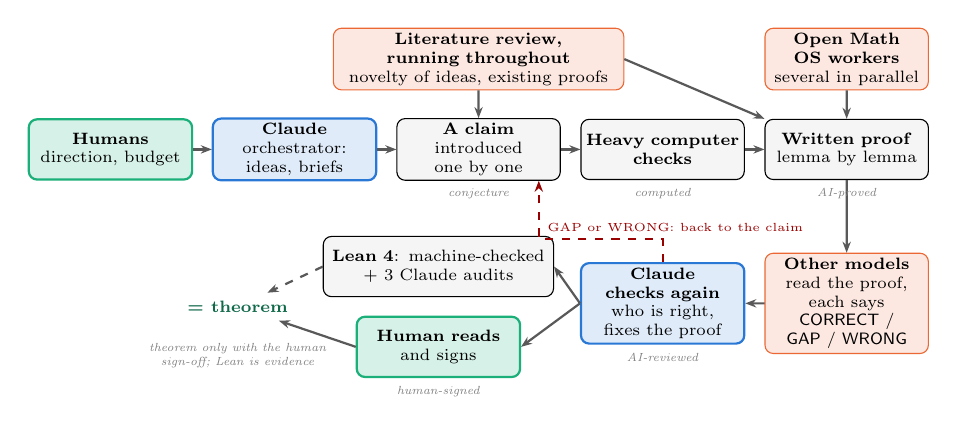
\begin{tikzpicture}[scale=0.85,transform shape,
      st/.style={draw,rounded corners=3pt,align=center,inner sep=2pt,
                 text width=23mm,minimum height=9mm,font=\scriptsize,fill=gray!8},
      ag/.style={st,fill=asymorange!15,draw=asymorange},
      cl/.style={st,fill=symblue!15,draw=symblue,thick},
      hu/.style={st,fill=atomgreen!18,draw=atomgreen,thick},
      gr/.style={font=\tiny\itshape,text=gray},
      fl/.style={-{Stealth[length=4pt]},thick,gray!70!black},
      fb/.style={-{Stealth[length=4pt]},thick,dashed,red!60!black}]
    % top row, left to right
    \node[hu] (H)  at (0,0)     {\textbf{Humans}\\ direction, budget};
    \node[cl] (O)  at (2.75,0)  {\textbf{Claude}\\ orchestrator:\\ ideas, briefs};
    \node[st] (C)  at (5.5,0)   {\textbf{A claim}\\ introduced one by one};
    \node[st] (X)  at (8.25,0)  {\textbf{Heavy computer}\\ \textbf{checks}};
    \node[st] (P)  at (11,0)    {\textbf{Written proof}\\ lemma by lemma};
    % helpers above
    \node[ag,text width=42mm] (L)  at (5.5,1.35)
      {\textbf{Literature review, running throughout}\\ novelty of ideas, existing proofs};
    \node[ag] (W)  at (11,1.35)   {\textbf{Open Math OS workers}\\ several in parallel};
    % bottom row, right to left
    \node[ag] (R)  at (11,-2.3)   {\textbf{Other models}\\ read the proof,\\ each says\\ \textsf{CORRECT / GAP / WRONG}};
    \node[cl] (A)  at (8.25,-2.3) {\textbf{Claude checks again}\\ who is right,\\ fixes the proof};
    \node[st,text width=33mm] (K)  at (4.9,-1.75) {\textbf{Lean 4}: machine-checked\\ + 3 Claude audits};
    \node[hu] (S)  at (4.9,-2.95) {\textbf{Human reads}\\ and signs};
    \node[font=\scriptsize\bfseries,text=atomgreen!60!black] (T) at (1.9,-2.35) {= theorem};
    % flow
    \draw[fl] (H) -- (O); \draw[fl] (O) -- (C); \draw[fl] (C) -- (X); \draw[fl] (X) -- (P);
    \draw[fl] (L) -- (C); \draw[fl] (L.east) -- (P.north west);
    \draw[fl] (W) -- (P);
    \draw[fl] (P) -- (R); \draw[fl] (R) -- (A);
    \draw[fl] (A.west) -- (K.east); \draw[fl] (A.west) -- (S.east);
    \draw[fl,dashed] (K.west) -- (T); \draw[fl] (S.west) -- (T);
    \draw[fb] (A.north) -- ++(0,0.35) -| node[pos=0.6,right,font=\tiny,text=red!60!black,align=left]{GAP or WRONG: back to the claim} ([xshift=9mm]C.south);
    % grades of the claim ledger
    \node[gr,below=0pt of C] {conjecture};
    \node[gr,below=0pt of X] {computed};
    \node[gr,below=0pt of P] {AI-proved};
    \node[gr,below=0pt of A] {AI-reviewed};
    \node[gr,below=0pt of S] {human-signed};
    \node[gr,below=6pt of T,align=center] {theorem only with the human\\ sign-off; Lean is evidence};
  \end{tikzpicture}

  \vspace{1pt}
  {\scriptsize
  \textcolor{atomgreen}{\rule{7pt}{7pt}} humans \quad
  \textcolor{symblue}{\rule{7pt}{7pt}} Claude (orchestrator) \quad
  \textcolor{asymorange}{\rule{7pt}{7pt}} other AI agents and models \quad
  \textcolor{gray!45}{\rule{7pt}{7pt}} claims, checks and proofs \par}

  \vspace{3pt}
  \raggedright\scriptsize
  \begin{itemize}\setlength{\itemsep}{0pt}
    \item Three models read the main proof in the first round; the other proofs had one or two AI readers each.
    \item Open Math OS agents and separate Claude sessions work from briefs of the orchestrating Claude
      session, which reads what they return and recompiles every Lean file before the file counts.
    \item Everything is recorded: a journal of every work block, a ledger of claims, the brief of every
      delegated run; Open Math OS runs are logged automatically.
    \item The ledger says for every claim which AI produced it, how it was checked, and whether a human signed it.
  \end{itemize}
\end{frame}

% 19 -----------------------------------------------------------------
% v2 (B-M1, B-M2): this frame now follows Section 1.4 and "The result on one page" of the report.
%  - "G. P\'olya, Acta Math. (1937)" is in no reference list of the project and is removed; the line keeps
%    the two OEIS sequences. (The report cites Robinson, Harary and Balaban, Tetrahedron 32 (1976), for the
%    cyclic group at a carbon, and P\'olya's paper of 1936 for the equation of A000625; there was no room
%    for them on this frame.)
%  - "Ours ...: the residue for all prime powers" contradicted the report: the residue is classical as a
%    statement. The last paragraph is now the report's list of what is new and what is not.
%  - Added, because the report credits them and the deck uses them: the shape of the smallest orbits
%    (Konvalinka); the classical congruence (through Granville's survey); Smith and Wildon (the method of
%    the lattice-path proof, which the frame "Three more proofs" now shows).
%  - "our second, algebraic proof" -> "the algebraic proof" (it is one of three further proofs).
%  The frame is set in \scriptsize so that it fits.
\begin{frame}{What was known, and references}
  \scriptsize
  \begin{itemize}\setlength{\itemsep}{0pt}
    \item \textbf{$p=2$, class size $2^{\mu}$ (``mutability'') and the series with a second variable:}
      I.~M.~H.~Etherington, \emph{Proc.\ Roy.\ Soc.\ Edinburgh} 59 (1939--40) 153--162.
    \item \textbf{$p=q=2$, exact valuation by orbits:} E.~Deutsch, B.~E.~Sagan,
      \emph{J.\ Number Theory} 117 (2006) 191--215. Weighted version: A.~Postnikov,
      B.~E.~Sagan, \emph{J.\ Combin.\ Theory Ser.\ A} 114 (2007) 970--977.
    \item \textbf{$q=p^k$, formula by factorials; divisibility by orbits of the full
      symmetric group; the shape of the smallest orbits:} M.~Konvalinka,
      \emph{J.\ Combin.\ Theory Ser.\ A} 114 (2007) 1089--1100.
    \item \textbf{$p=2$, the minimal trees again, as most balanced evolutionary trees:}
      S.~J.~Kersting, M.~Fischer, \emph{Math.\ Biosci.} (2021),
      doi:10.1016/j.mbs.2021.108690. No mention of Catalan numbers.
    \item \textbf{Both formulas as statements about binomial coefficients:} Kummer; Anton, Stickelberger,
      Hensel; quoted from A.~Granville, \emph{CMS Conf.\ Proc.}\ 20 (1997) 253--276.
    \item \textbf{Generating functions modulo prime powers, via $\sum z^{p^n}$:}
      M.~Kauers, C.~Krattenthaler, T.~W.~M\"uller, \emph{Electron.\ J.\ Combin.} 18(2)
      (2012) P37; C.~Krattenthaler, T.~W.~M\"uller, \emph{Aequationes Math.} 99 (2025)
      2505--2547. The starting point, modulo $p$, of the algebraic proof.
    \item \textbf{The method of the lattice-path proof:} J.~H.~Smith, \emph{Graphs Combin.} 9 (1993)
      293--304; M.~Wildon, MathOverflow, answer 234272 (2016).
    \item \textbf{Trees up to rotation at each node:} sequences OEIS A000625 (alkyl groups), A001190.
  \end{itemize}
  \textbf{New, as far as we know:} cyclic rotations, a $p$-group, used for this theorem, for every
  prime power; the smallest classes in base $p$ with the depth condition; their count modulo $p$ by
  collapsing cherries, and with it the exactness and the residue from tree symmetries.
  \textbf{Not new:} both formulas as statements; the divisibility by a group action and the shape of the
  smallest orbits; everything for $p=2$; the classes under rotation as objects; the fixed-point principle.
  \emph{Not a certificate of novelty.} These sources were read by AI systems, not by us.
\end{frame}

% ---- backup slides (added 2026-11-14) --------------------------------
\begin{frame}{Backup: a carry is two equal blocks fusing}
  \centering
  % v2 (B-R12): fig_fusion_v2 no longer names "a binary counter" and "a buddy memory allocator", which are not
  % in the report; its last line reads "merging binomial queues; sand that topples in pairs" (report,
  % Section 5, items 6 and 11).
  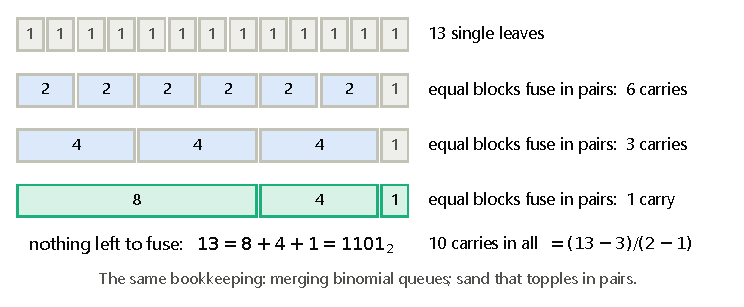
\includegraphics[width=0.95\textwidth]{figures/fig_fusion_v2.pdf}\\[4pt]
  \begin{minipage}{0.93\textwidth}\small
  % v2 (B-M11): "In the proof, each fusion is a cherry of $p$ equal subtrees collapsing." is true of the
  % accounting proof only; in the main proof the cherries that collapse are $p$ distinct labels. The sentence
  % is now the report's (Section 5, item 6).
  For a tree with $13$ leaves: $12$ nodes, at most $10$ of them symmetric (one per carry), so at least $2$
  asymmetric. Each fusion is a carry.
  \end{minipage}
\end{frame}

% v2 (B-R13 to B-R17): the five backup slides that follow are compiled only with \extrabackuptrue (see the
% top of the file): their worked examples are not written in the report.
\ifextrabackup

\begin{frame}{Backup: tree $=$ cut of an interval $=$ cut into balls}
  \centering
  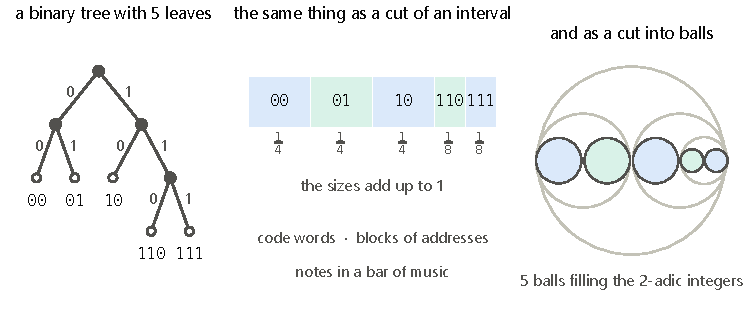
\includegraphics[width=0.95\textwidth]{figures/fig_balls.pdf}\\[4pt]
  \begin{minipage}{0.93\textwidth}\small
  % v2 (B-R13): "; our rotations are isometries of them" is removed (true, and not in the report).
  The Catalan number $C_{m-1}$ counts the ways to cut the $2$-adic integers into $m$ balls.
  In a computer the same cuts are prefix codes and blocks of addresses; for $q=2^8$ the
  blocks are aligned to whole bytes.
  \end{minipage}
\end{frame}

\begin{frame}{Backup: polymers ($p=3$)}
  \centering
  % v2 (B-M15): fig_dendrimer_v2 says "a most symmetric one" (there are two), not "the"
  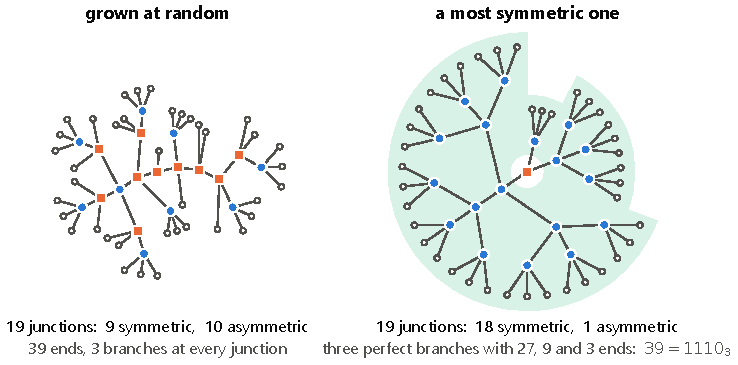
\includegraphics[width=0.8\textwidth]{figures/fig_dendrimer_v2.pdf}\\[2pt]
  \begin{minipage}{0.95\textwidth}\small
  A molecule with $m$ ends can be perfectly branched only if $m$ is a power of $p$; otherwise it is $t$
  junctions short. In the classical theory of polymer branching, Stockmayer's combinatorial factor for
  $n$ units with $f$ reactive groups is the Fuss--Catalan number for $q=f-1$ divided by the number of
  free groups (units with three reactive groups give the Catalan numbers).
  \end{minipage}
\end{frame}

\begin{frame}{Backup: cut a triangle ($p=3$)}
  \centering
  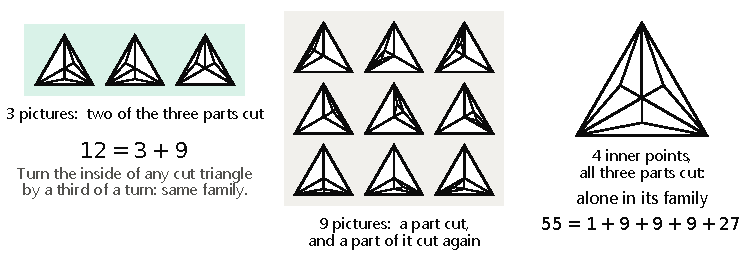
\includegraphics[width=0.95\textwidth]{figures/fig_triangles.pdf}\\[4pt]
  \begin{minipage}{0.93\textwidth}\small
  % v2 (B-R15): "the twin of \emph{tert}-butyl" is now said in the report's words (Section 2.2: the class of
  % size 1 is the complete tree of height 2, which is tert-butyl).
  Put a point inside a triangle, join it to the corners, repeat. Turning the inside of a cut triangle by a
  third of a turn is our rotation. The picture that stands alone is the complete tree of height $2$, the
  tree of \emph{tert}-butyl.
  \end{minipage}
\end{frame}

\begin{frame}{Backup: light, doubling and mixing ($p=2$)}
  \centering
  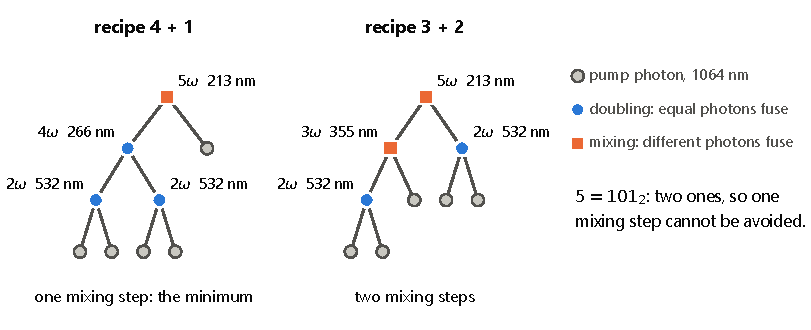
\includegraphics[width=0.9\textwidth]{figures/fig_laser.pdf}\\[2pt]
  \begin{minipage}{0.95\textwidth}\small
  A nonlinear crystal fuses two photons into one. In the history of any photon of the $m$-th harmonic, at
  % v2 (B-R16): "Both recipes for the fifth harmonic are in use." is removed: the report has no source for it.
  % (The wavelengths in the figure are not in the report either; this slide is compiled only with
  % \extrabackuptrue.)
  least $(\text{number of ones of } m)-1$ fusions are mixings of two different photons.
  {\footnotesize (A real apparatus can reuse a beam; then the count can drop, first at
  $m=15$.)}
  \end{minipage}
\end{frame}

\begin{frame}{Backup: prime powers as sand on a ring}
  \centering
  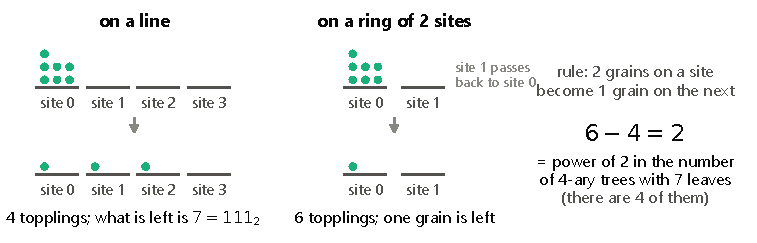
\includegraphics[width=0.92\textwidth]{figures/fig_sand.pdf}\\[4pt]
  \begin{minipage}{0.93\textwidth}\small
  For $q=p^k$: $p$ grains on a site topple into one grain on the next site, on a ring of $k$ sites.
  The power of $p$ in $\Cq$ is the number of topplings on the ring minus the number on a line.
  \end{minipage}
\end{frame}
\fi % v2: end of \ifextrabackup

\end{document}
